\chapter{Gestures as a communication tool}

\begin{wrapfigure}{r}{0.5\textwidth}
  \begin{center}
    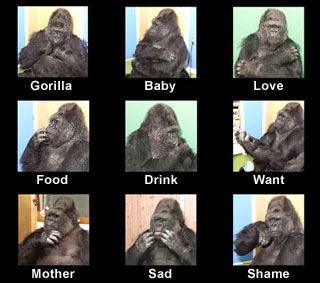
\includegraphics[width=0.48\textwidth]{img/gorillagesture.jpg}
  \end{center}
  \caption{Koko Gorilla Sign Language}
\end{wrapfigure}

\section{Origin of Gestures}
Gestures have been been used as a communication tool since before speech was invented. Gestures convey information rapidly in early human culture. \cite{nonverbalgesture} Gestures such as point and facial gestures such as fear would convey danger with a location. Although not very detailed, it quickly conveyed to the rest of early humans that danger was close. \cite{nonverbalgesture}

Gorillas have been seen to use gestures and can be taught new ones. Koko the gorilla is a prime example of how gestures may have been used in early human development. She could use gestures to convey emotions and needs. \cite{koko}

Gestures were a vital part of early human communication and continue to be a communication tool in other primate troops.

\section{Modern Gestures}

Modern gestures differ from culture to culture, so I'll be talking about the gestures used in the western world.

\begin{wrapfigure}{r}{0.5\textwidth}
  \begin{center}
    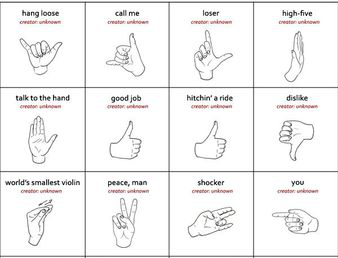
\includegraphics[width=0.48\textwidth]{img/handgesture.png}
  \end{center}
  \caption{Hand Gestures}
\end{wrapfigure}

Gestures used today are extremely common place.  A single gesture might have multiple meaning given the context its used in. An example is the stop gesture. The stop gesture involves facing your palm of your hand toward the user with fingers placed upwards and close together. This gesture is used to say stop, talk to the hand, giving way to a pedestrian while driving and thanking another driver who has given way to you.

Modern gestures are used everywhere to convey a message quickly. A gesture becomes common place due to many reasons, mostly cultural. A thumbs up in the western world is a common gesture to say 'good job' or just to say 'OK'. This is a common gesture used in the western world but in the middle east and central Africa it is used to convey frustration with another person by directing the gesture towards them as an insult.

